\documentclass[UTF8]{ctexart}
\usepackage{multirow}
\usepackage{geometry}
\usepackage{natbib}
\usepackage{booktabs}
\usepackage{hyperref} 
\usepackage{amsmath}
\usepackage{amsfonts}
\usepackage{eucal}
\usepackage{cancel}
\usepackage{amssymb}
\usepackage{calligra}
\usepackage{multirow}
\usepackage{bm}
\usepackage{ulem}
\usepackage{graphicx}
\usepackage{subfigure}
\usepackage{float}
\usepackage{pgf,tikz,pgfplots}
\pgfplotsset{compat=1.15}
\usepackage{mathrsfs}
\usetikzlibrary{arrows}
\begin{document}
% \definecolor{uququq}{rgb}{0.25098039215686274,0.25098039215686274,0.25098039215686274}
% \definecolor{uuuuuu}{rgb}{0.26666666666666666,0.26666666666666666,0.26666666666666666}
% \definecolor{ududff}{rgb}{0.30196078431372547,0.30196078431372547,1}
% \begin{tikzpicture}[line cap=round,line join=round,>=triangle 45,x=1cm,y=1cm]
% \clip(-6.908850488354623,-5.954387678437262) rectangle (9.289496619083398,5.615860255447021);
% \draw [line width=2pt] (-5,0)-- (5,0);
% \draw [line width=2pt] (0,5)-- (0,-5);
% \draw [rotate around={-41.3947648478864:(-0.6685499624342615,0.5892975206611561)},line width=2pt,color=uququq,fill=uququq,fill opacity=0.53] (-0.6685499624342615,0.5892975206611561) ellipse (1.2218494969258322cm and 0.8358741370623162cm);
% \draw [rotate around={-138.6052351521136:(0.6685499624342613,0.5892975206611563)},line width=2pt,color=uququq,fill=uququq,fill opacity=0.66] (0.6685499624342613,0.5892975206611563) ellipse (1.2218494969258322cm and 0.8358741370623162cm);
% \draw [rotate around={41.3947648478864:(-0.6685499624342615,-0.5892975206611561)},line width=2pt,color=uququq,fill=uququq,fill opacity=0.72] (-0.6685499624342615,-0.5892975206611561) ellipse (1.2218494969258322cm and 0.8358741370623162cm);
% \draw [rotate around={138.6052351521136:(0.6685499624342616,-0.589297520661156)},line width=2pt,color=uququq,fill=uququq,fill opacity=0.69] (0.6685499624342616,-0.589297520661156) ellipse (1.2218494969258322cm and 0.8358741370623162cm);
% \draw (1.7192486851990987,3.0538767843726444) node[anchor=north west] {$d_{xy},d_{yz},d_{zx}$};
% \begin{scriptsize}
% \draw [fill=ududff] (-5,0) circle (2.5pt);
% \draw [fill=ududff] (5,0) circle (2.5pt);
% \draw [fill=ududff] (0,5) circle (2.5pt);
% \draw [fill=ududff] (0,-5) circle (2.5pt);
% \draw [fill=uuuuuu] (0,0) circle (2pt);
% \end{scriptsize}
% \end{tikzpicture}

% \definecolor{uuuuuu}{rgb}{0.26666666666666666,0.26666666666666666,0.26666666666666666}
% \definecolor{xdxdff}{rgb}{0.49019607843137253,0.49019607843137253,1}
% \definecolor{uququq}{rgb}{0.25098039215686274,0.25098039215686274,0.25098039215686274}
% \definecolor{ududff}{rgb}{0.30196078431372547,0.30196078431372547,1}

% \begin{figure}[]
%     \centering
%     \resizebox{\textwidth}{!}{
%     \begin{tikzpicture}[line cap=round,line join=round,>=triangle 45,x=0.4cm,y=0.4cm]
%         \clip(-7.568420055431509,-14.648982459713856) rectangle (30.651216037856322,15.468248877500034);
%         \draw [line width=2pt] (-5,0)-- (5,0);
%         \draw [line width=2pt] (0,5)-- (0,-5);
%         \draw [rotate around={-50.05724853255913:(-0.585,0.685)},line width=2pt,color=uququq,fill=uququq,fill opacity=0.53] (-0.585,0.685) ellipse (0.9009667929793787 and 0.4102330582139209);
%         \draw [rotate around={-129.94275146744084:(0.585,0.685)},line width=2pt,color=uququq,fill=uququq,fill opacity=0.66] (0.585,0.685) ellipse (0.9009667929793787 and 0.4102330582139209);
%         \draw [rotate around={50.05724853255913:(-0.585,-0.685)},line width=2pt,color=uququq,fill=uququq,fill opacity=0.72] (-0.585,-0.685) ellipse (0.9009667929793787 and 0.4102330582139209);
%         \draw [rotate around={129.94275146744087:(0.585,-0.685)},line width=2pt,color=uququq,fill=uququq,fill opacity=0.69] (0.585,-0.685) ellipse (0.9009667929793787 and 0.4102330582139209);
%         \draw (2.114941726218458,4.520121475389473) node[anchor=north west] {$\mathbf{d_{xy},d_{yz},d_{zx}}$};
%         \draw [line width=2pt] (7,0)-- (17,0);
%         \draw [line width=2pt] (12,5)-- (12,-5);
%         \draw [line width=2pt] (19,0)-- (29,0);
%         \draw [line width=2pt] (24,5)-- (24,-5);
%         \draw [rotate around={90:(12,1.1638436934424887)},line width=2pt,fill=black,fill opacity=0.39] (12,1.1638436934424887) ellipse (1.2260171011811196 and 0.38546827317293436);
%         \draw [rotate around={180:(10.83615630655751,0)},line width=2pt,fill=black,fill opacity=0.2] (10.83615630655751,0) ellipse (1.2260171011811196 and 0.38546827317293436);
%         \draw [rotate around={-90:(12,-1.1638436934424887)},line width=2pt,fill=black,fill opacity=0.2] (12,-1.1638436934424887) ellipse (1.2260171011811196 and 0.38546827317293436);
%         \draw [rotate around={0:(13.16384369344249,0)},line width=2pt,fill=black,fill opacity=0.2] (13.16384369344249,0) ellipse (1.2260171011811196 and 0.38546827317293436);
%         \draw [rotate around={0:(24.00254899481813,0)},line width=2pt,fill=black,fill opacity=0.2] (24.00254899481813,0) ellipse (1.6839389847634159 and 0.7648916185947887);
%         \draw [rotate around={90:(24,1.4398026937089552)},line width=2pt,fill=black,fill opacity=0.2] (24,1.4398026937089552) ellipse (1.4398026937087463 and 0.7020750078174347);
%         \draw [rotate around={-90:(24,-1.4398026937089552)},line width=2pt,fill=black,fill opacity=0.2] (24,-1.4398026937089552) ellipse (1.4398026937087463 and 0.7020750078174347);
%         \draw (14.130215120592297,4.520121475389473) node[anchor=north west] {$\mathbf{d_{x^{2}-y^{2}}}$};
%         \draw (26.105964589326746,4.520121475389473) node[anchor=north west] {$\mathbf{d_{z^{2}}}$};
%         \begin{scriptsize}
%         \draw [fill=ududff] (-5,0) circle (2.5pt);
%         \draw [fill=ududff] (5,0) circle (2.5pt);
%         \draw [fill=ududff] (0,5) circle (2.5pt);
%         \draw [fill=ududff] (0,-5) circle (2.5pt);
%         \draw [fill=ududff] (7,0) circle (2.5pt);
%         \draw [fill=ududff] (17,0) circle (2.5pt);
%         \draw [fill=ududff] (12,5) circle (2.5pt);
%         \draw [fill=ududff] (12,-5) circle (2.5pt);
%         \draw [fill=xdxdff] (19,0) circle (2.5pt);
%         \draw [fill=xdxdff] (29,0) circle (2.5pt);
%         \draw [fill=ududff] (24,5) circle (2.5pt);
%         \draw [fill=ududff] (24,-5) circle (2.5pt);
%         \draw [fill=uuuuuu] (12,0) circle (2pt);
%         \end{scriptsize}
%         \end{tikzpicture}
%     }
%     \vspace*{-3cm}
%     \caption{轨道提u}
%     \label{}
% \end{figure}


    
% \begin{table}[!htbp]
%     \caption{八面体配合物的高自旋态与低自旋态}
%     \label{tab:dog}
%     \resizebox{\textwidth}{!}{
%     \begin{tabular}{c|c|c|c|c|c|c|c|c}
%         \toprule
%         \multirow{2}*{$n_{d}$(d电子数)}&\multicolumn{4}{|c|}{高自旋态}&\multicolumn{4}{|c}{低自旋态}\\
%         \cline{2-9}
%         &$t_{2g}$&$e_{g}$&n&p&$t_{2g}$&$e_{g}$&n&p\\
%         \midrule
%         1&\sout{↑\ }\ \sout{\ \ }\ \sout{\ \ }&\sout{\ \ }\ \sout{\ \ }&1&1.73&&&&\\
%         \hline
%         2&\sout{↑\ }\ \sout{↑\ }\ \sout{\ \ }&\sout{\ \ }\ \sout{\ \ }&2&2.83&&&&\\
%         \hline
%         3&\sout{↑\ }\ \sout{↑\ }\ \sout{↑\ }&\sout{\ \ }\ \sout{\ \ }&3&3.87&&&&\\
%         \hline
%         4&\sout{↑\ }\ \sout{↑\ }\ \sout{↑\ }&\sout{↑\ }\ \sout{\ \ }&4&4.90&\sout{↑↓}\ \sout{↑\ }\ \sout{↑\ }&\sout{\ \ }\ \sout{\ \ }&2&2.83\\
%         \hline
%         5&\sout{↑\ }\ \sout{↑\ }\ \sout{↑\ }&\sout{↑\ }\ \sout{↑\ }&5&5.92&\sout{↑↓}\ \sout{↑↓}\ \sout{↑\ }&\sout{\ \ }\ \sout{\ \ }&1&1.73\\
%         \hline
%         6&\sout{↑↓}\ \sout{↑\ }\ \sout{↑\ }&\sout{↑\ }\ \sout{↑\ }&4&4.90&\sout{↑↓}\ \sout{↑↓}\ \sout{↑↓}&\sout{\ \ }\ \sout{\ \ }&0&0\\
%         \hline
%         7&\sout{↑↓}\ \sout{↑↓}\ \sout{↑\ }&\sout{↑\ }\ \sout{↑\ }&3&3.87&\sout{↑↓}\ \sout{↑↓}\ \sout{↑↓}&\sout{↑\ }\ \sout{\ \ }&1&1.73\\
%         \hline
%         8&\sout{↑↓}\ \sout{↑↓}\ \sout{↑↓}&\sout{↑\ }\ \sout{↑\ }&2&2.83&&&&\\
%         \hline
%         9&\sout{↑↓}\ \sout{↑↓}\ \sout{↑↓}&\sout{↑↓}\ \sout{↑\ }&1&1.73&&&&\\
%         \bottomrule
%     \end{tabular}
%     }
% \end{table}

% \begin{figure}[]
%     \centering
%     \resizebox{\textwidth}{!}{
%         \begin{tikzpicture}[line cap=round,line join=round,>=triangle 45,x=3cm,y=3cm]
%             \clip(-4.880291166623681,-2.3485074264249626) rectangle (5.396326222588918,6.000589473883519);
%             \draw [->,line width=2pt] (-1,2) -- (1,2);
%             \draw [->,line width=2pt] (1,1.5) -- (-1,1.5);
%             \draw (-0.31386821851793875,1.4436796223977102) node[anchor=north west] {\parbox{3.167610477296026 cm}{\Huge 温度 \\ 压强 \\ 光照}};
%             \draw [line width=2pt] (-2.5,2.5)-- (-2,2.5);
%             \draw [line width=2pt] (-3.5,2.5)-- (-3,2.5);
%             \draw [line width=2pt] (3.5,2.5)-- (3,2.5);
%             \draw [line width=2pt] (2.5,2.5)-- (2,2.5);
%             \draw [line width=2pt] (-2.5,1)-- (-3,1);
%             \draw [line width=2pt] (-2,1)-- (-1.5,1);
%             \draw [line width=2pt] (-3.5,1)-- (-4,1);
%             \draw [line width=2pt] (2.5,1)-- (3,1);
%             \draw [line width=2pt] (2,1)-- (1.5,1);
%             \draw [line width=2pt] (3.5,1)-- (4,1);
%             \draw [->,line width=2pt] (-3.9,0.8) -- (-3.9,1.2);
%             \draw [->,line width=2pt] (-3.6,1.2) -- (-3.6,0.8);
%             \draw [->,line width=2pt] (-2.9,0.8) -- (-2.9,1.2);
%             \draw [->,line width=2pt] (-2.6,1.2) -- (-2.6,0.8);
%             \draw [->,line width=2pt] (-1.9,0.8) -- (-1.9,1.2);
%             \draw [->,line width=2pt] (-1.6,1.2) -- (-1.6,0.8);
%             \draw [->,line width=2pt] (1.6,0.8) -- (1.6,1.2);
%             \draw [->,line width=2pt] (1.9,1.2) -- (1.9,0.8);
%             \draw [->,line width=2pt] (2.7,0.8) -- (2.7,1.2);
%             \draw [->,line width=2pt] (3.7,0.8) -- (3.7,1.2);
%             \draw [->,line width=2pt] (2.2,2.3) -- (2.2,2.7);
%             \draw [->,line width=2pt] (3.2,2.3) -- (3.2,2.7);
%             \draw (-3.0680028808603987,0.5637246165935542) node[anchor=north west] {\parbox{5 cm}{\Huge 低自旋态 \\ S=0}};
%             \draw (2.4107645957534545,0.5532489617625523) node[anchor=north west] {\parbox{5 cm}{\Huge 高自旋态 \\ S=2}};
%             \end{tikzpicture}
%     }
%     \vspace*{-3cm}
%     \caption{轨道提u}
%     \label{}
% \end{figure}
\definecolor{qqwuqq}{rgb}{0,0.39215686274509803,0}
\definecolor{zzttqq}{rgb}{0.6,0.2,0}
\definecolor{fuqqzz}{rgb}{0.9568627450980393,0,0.6}
\definecolor{xdxdff}{rgb}{0.49019607843137253,0.49019607843137253,1}
\definecolor{qqwuqq}{rgb}{0,0.39215686274509803,0}
\definecolor{uuuuuu}{rgb}{0.26666666666666666,0.26666666666666666,0.26666666666666666}
\definecolor{zzttqq}{rgb}{0.6,0.2,0}
\definecolor{ududff}{rgb}{0.30196078431372547,0.30196078431372547,1}

\begin{figure}[htbp]
    \centering
    \resizebox{\textwidth}{!}{
    \subfigure[]{
        \centering
        \resizebox{\textwidth}{!}{
    \begin{tikzpicture}[line cap=round,line join=round,>=triangle 45,x=1cm,y=1cm]
        \clip(-7.194992758719219,-5.824543307427976) rectangle (7.195799831044691,5.830809368579352);
        \draw [line width=2pt] (-2,1)-- (-2,0);
        \draw [line width=2pt] (-2,0)-- (-3.002633760461551,-0.7922258573916472);
        \draw [line width=2pt] (-2,0)-- (-1.7687124950169182,-1.01522367644791);
        \draw [line width=2pt] (-2,0)-- (-0.9956533889552205,-0.3908297830903744);
        \draw [line width=2pt] (2,1)-- (2,0);
        \draw [line width=2pt] (2,0)-- (0.9956533889552205,-0.3908297830903745);
        \draw [line width=2pt] (2,0)-- (1.768712495016918,-1.0152236764479101);
        \draw [line width=2pt] (2,0)-- (3.002633760461551,-0.7922258573916475);
        \draw [line width=2pt] (0,2)-- (0,-2);
        \begin{scriptsize}
        \draw [fill=xdxdff] (-2,0) circle (2.5pt);
        \draw [fill=fuqqzz] (-2,1) circle (2.5pt);
        \draw [fill=black] (-0.9956533889552205,-0.3908297830903744) circle (2.5pt);
        \draw [fill=zzttqq] (-1.7687124950169182,-1.01522367644791) circle (2.5pt);
        \draw [fill=qqwuqq] (-3.002633760461551,-0.7922258573916472) circle (2.5pt);
        \draw [fill=fuqqzz] (2,1) circle (2.5pt);
        \draw [fill=xdxdff] (2,0) circle (2.5pt);
        \draw [fill=fuqqzz] (2,1) circle (2.5pt);
        \draw [fill=xdxdff] (2,0) circle (2.5pt);
        \draw [fill=xdxdff] (2,0) circle (2.5pt);
        \draw [fill=black] (0.9956533889552205,-0.3908297830903745) circle (2.5pt);
        \draw [fill=xdxdff] (2,0) circle (2.5pt);
        \draw [fill=zzttqq] (1.768712495016918,-1.0152236764479101) circle (2.5pt);
        \draw [fill=xdxdff] (2,0) circle (2.5pt);
        \draw [fill=qqwuqq] (3.002633760461551,-0.7922258573916475) circle (2.5pt);
        \end{scriptsize}
        \end{tikzpicture}
        }
    }
    \subfigure[]{
        \centering
        \begin{tikzpicture}[line cap=round,line join=round,>=triangle 45,x=1cm,y=1cm]
            \clip(-2.6002252010650246,-4.6898893752016075) rectangle (5.259762267797396,1.2182891248828964);
            \fill[line width=2pt,color=zzttqq,fill=zzttqq,fill opacity=0.10000000149011612] (-1.4,-2.424871130596429) -- (-0.49411828718356193,-1.9352997555018803) -- (-1.1,-1.9052558883257653) -- cycle;
            \fill[line width=2pt,color=zzttqq,fill=zzttqq,fill opacity=0.10000000149011612] (1.4,-2.424871130596429) -- (0.49411828718356215,-1.9352997555018803) -- (1.1,-1.905255888325765) -- cycle;
            \fill[line width=2pt,color=zzttqq,fill=zzttqq,fill opacity=0.10000000149011612] (2.8,0) -- (1.9230778957942223,0.5397308885755209) -- (2.2,0) -- cycle;
            \draw [shift={(0,0)},line width=2pt,color=qqwuqq,fill=qqwuqq,fill opacity=0.10000000149011612] (0,0) -- (-120:0.226078258931805) arc (-120:0:0.226078258931805) -- cycle;
            \draw [line width=2pt] (-0.43301270189221924,0.25)-- (3.464101615137755,-2);
            \draw [line width=2pt] (0,0.5)-- (0,-4);
            \draw [line width=2pt] (0,0.5)-- (0,-4);
            \draw [line width=2pt,color=zzttqq] (-1.4,-2.424871130596429)-- (-0.49411828718356193,-1.9352997555018803);
            \draw [line width=2pt,color=zzttqq] (-0.49411828718356193,-1.9352997555018803)-- (-1.1,-1.9052558883257653);
            \draw [line width=2pt,color=zzttqq] (-1.1,-1.9052558883257653)-- (-1.4,-2.424871130596429);
            \draw [line width=2pt,color=zzttqq] (1.4,-2.424871130596429)-- (0.49411828718356215,-1.9352997555018803);
            \draw [line width=2pt,color=zzttqq] (0.49411828718356215,-1.9352997555018803)-- (1.1,-1.905255888325765);
            \draw [line width=2pt,color=zzttqq] (1.1,-1.905255888325765)-- (1.4,-2.424871130596429);
            \draw [line width=2pt,color=zzttqq] (2.8,0)-- (1.9230778957942223,0.5397308885755209);
            \draw [line width=2pt,color=zzttqq] (1.9230778957942223,0.5397308885755209)-- (2.2,0);
            \draw [line width=2pt,color=zzttqq] (2.2,0)-- (2.8,0);
            \draw [line width=2pt,dash pattern=on 1pt off 1pt] (-1.1,-1.9052558883257653)-- (0,0);
            \draw [line width=2pt,dash pattern=on 1pt off 1pt] (2.2,0)-- (0,0);
            \draw [shift={(0,0)},line width=2pt]  plot[domain=4.71238898038469:5.759586531581287,variable=\t]({1*0.6506244822866917*cos(\t r)+0*0.6506244822866917*sin(\t r)},{0*0.6506244822866917*cos(\t r)+1*0.6506244822866917*sin(\t r)});
            \draw (0.3538640489772274,-0.597872888535937) node[anchor=north west] {$\alpha$/2};
            \draw (0.1805373837961769,-3.416315183219106) node[anchor=north west] {m};
            \draw (3.17984228562479,-2.0673815715926693) node[anchor=north west] {m'};
            \draw (-0.2640831921030396,-0.03267724120642451) node[anchor=north west] {$\alpha$};
            \begin{scriptsize}
            \draw [fill=ududff] (-1.4,-2.424871130596429) circle (2.5pt);
            \draw [fill=ududff] (-0.49411828718356193,-1.9352997555018803) circle (2.5pt);
            \draw [fill=ududff] (-1.1,-1.9052558883257653) circle (2.5pt);
            \draw [fill=ududff] (1.4,-2.424871130596429) circle (2.5pt);
            \draw [fill=ududff] (0.49411828718356215,-1.9352997555018803) circle (2.5pt);
            \draw [fill=ududff] (1.1,-1.905255888325765) circle (2.5pt);
            \draw [fill=ududff] (2.8,0) circle (2.5pt);
            \draw [fill=ududff] (1.9230778957942223,0.5397308885755209) circle (2.5pt);
            \draw [fill=ududff] (2.2,0) circle (2.5pt);
            \draw [fill=uuuuuu] (0,0) circle (2pt);
            \end{scriptsize}
            \end{tikzpicture}
    }
    }
    \caption{}
    \label{}
\end{figure}

\begin{figure}[htbp]
    \centering
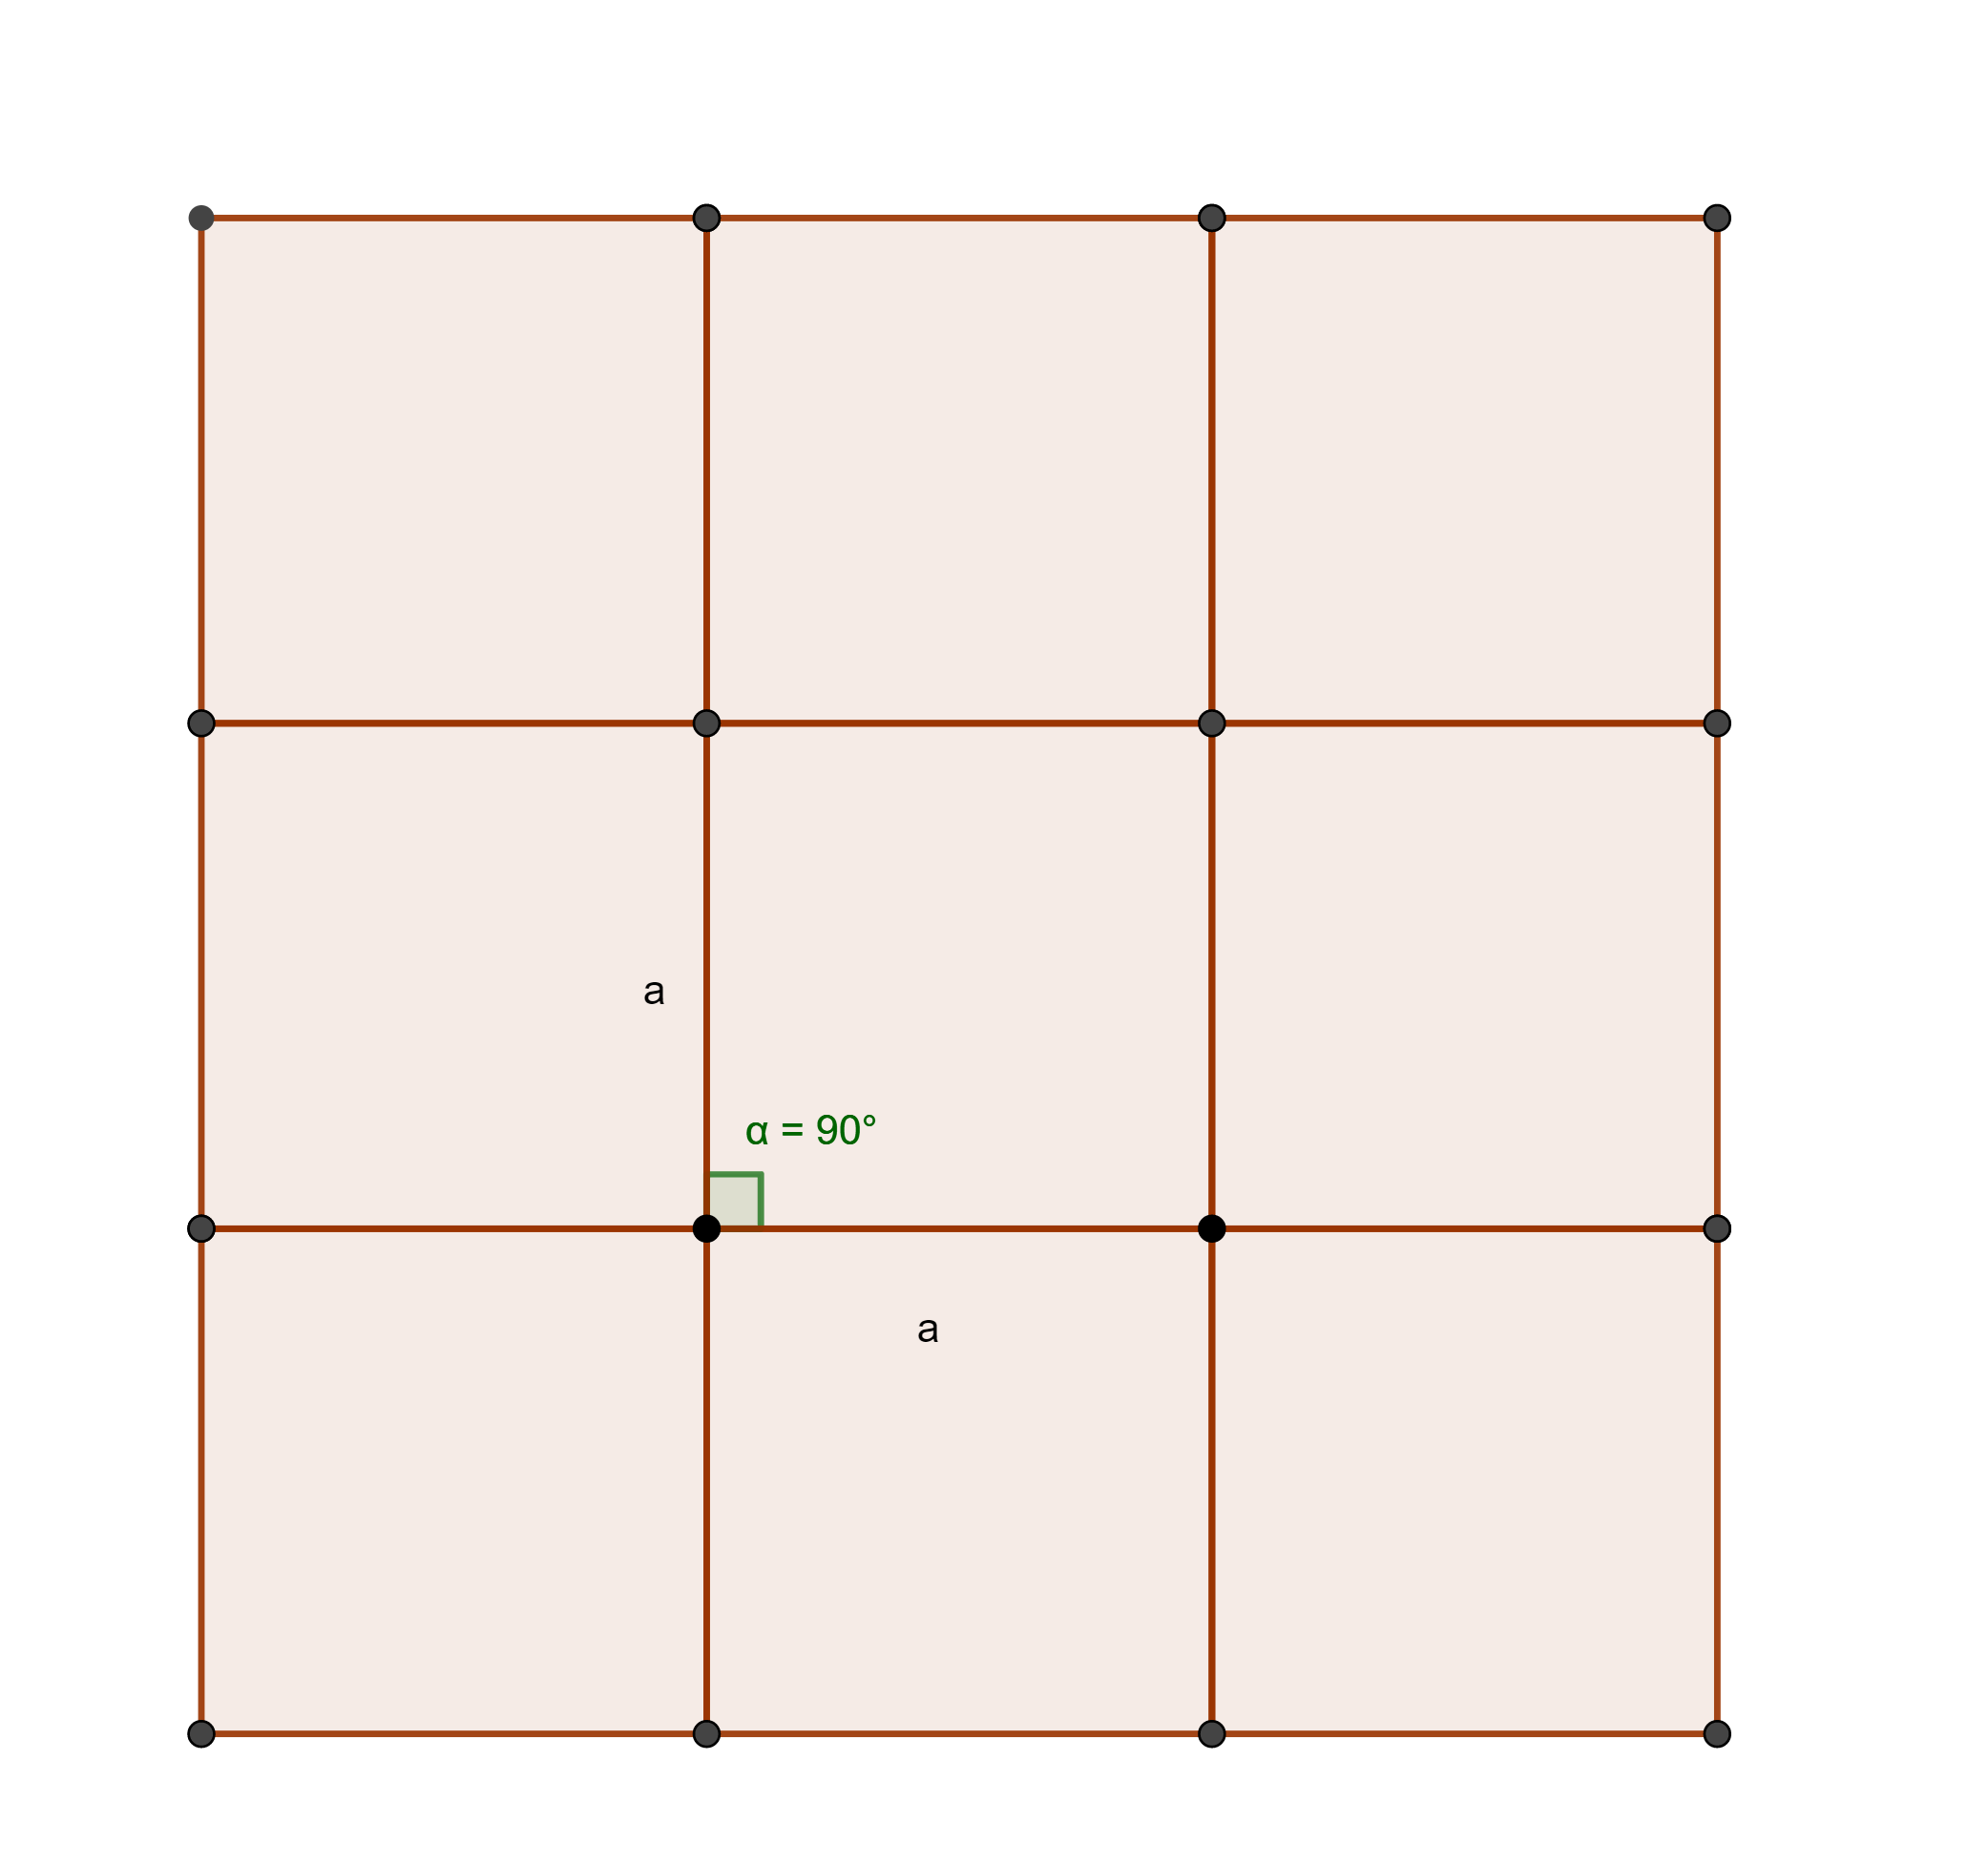
\includegraphics[width=0.4\textwidth]{./pic/p008-1.png}
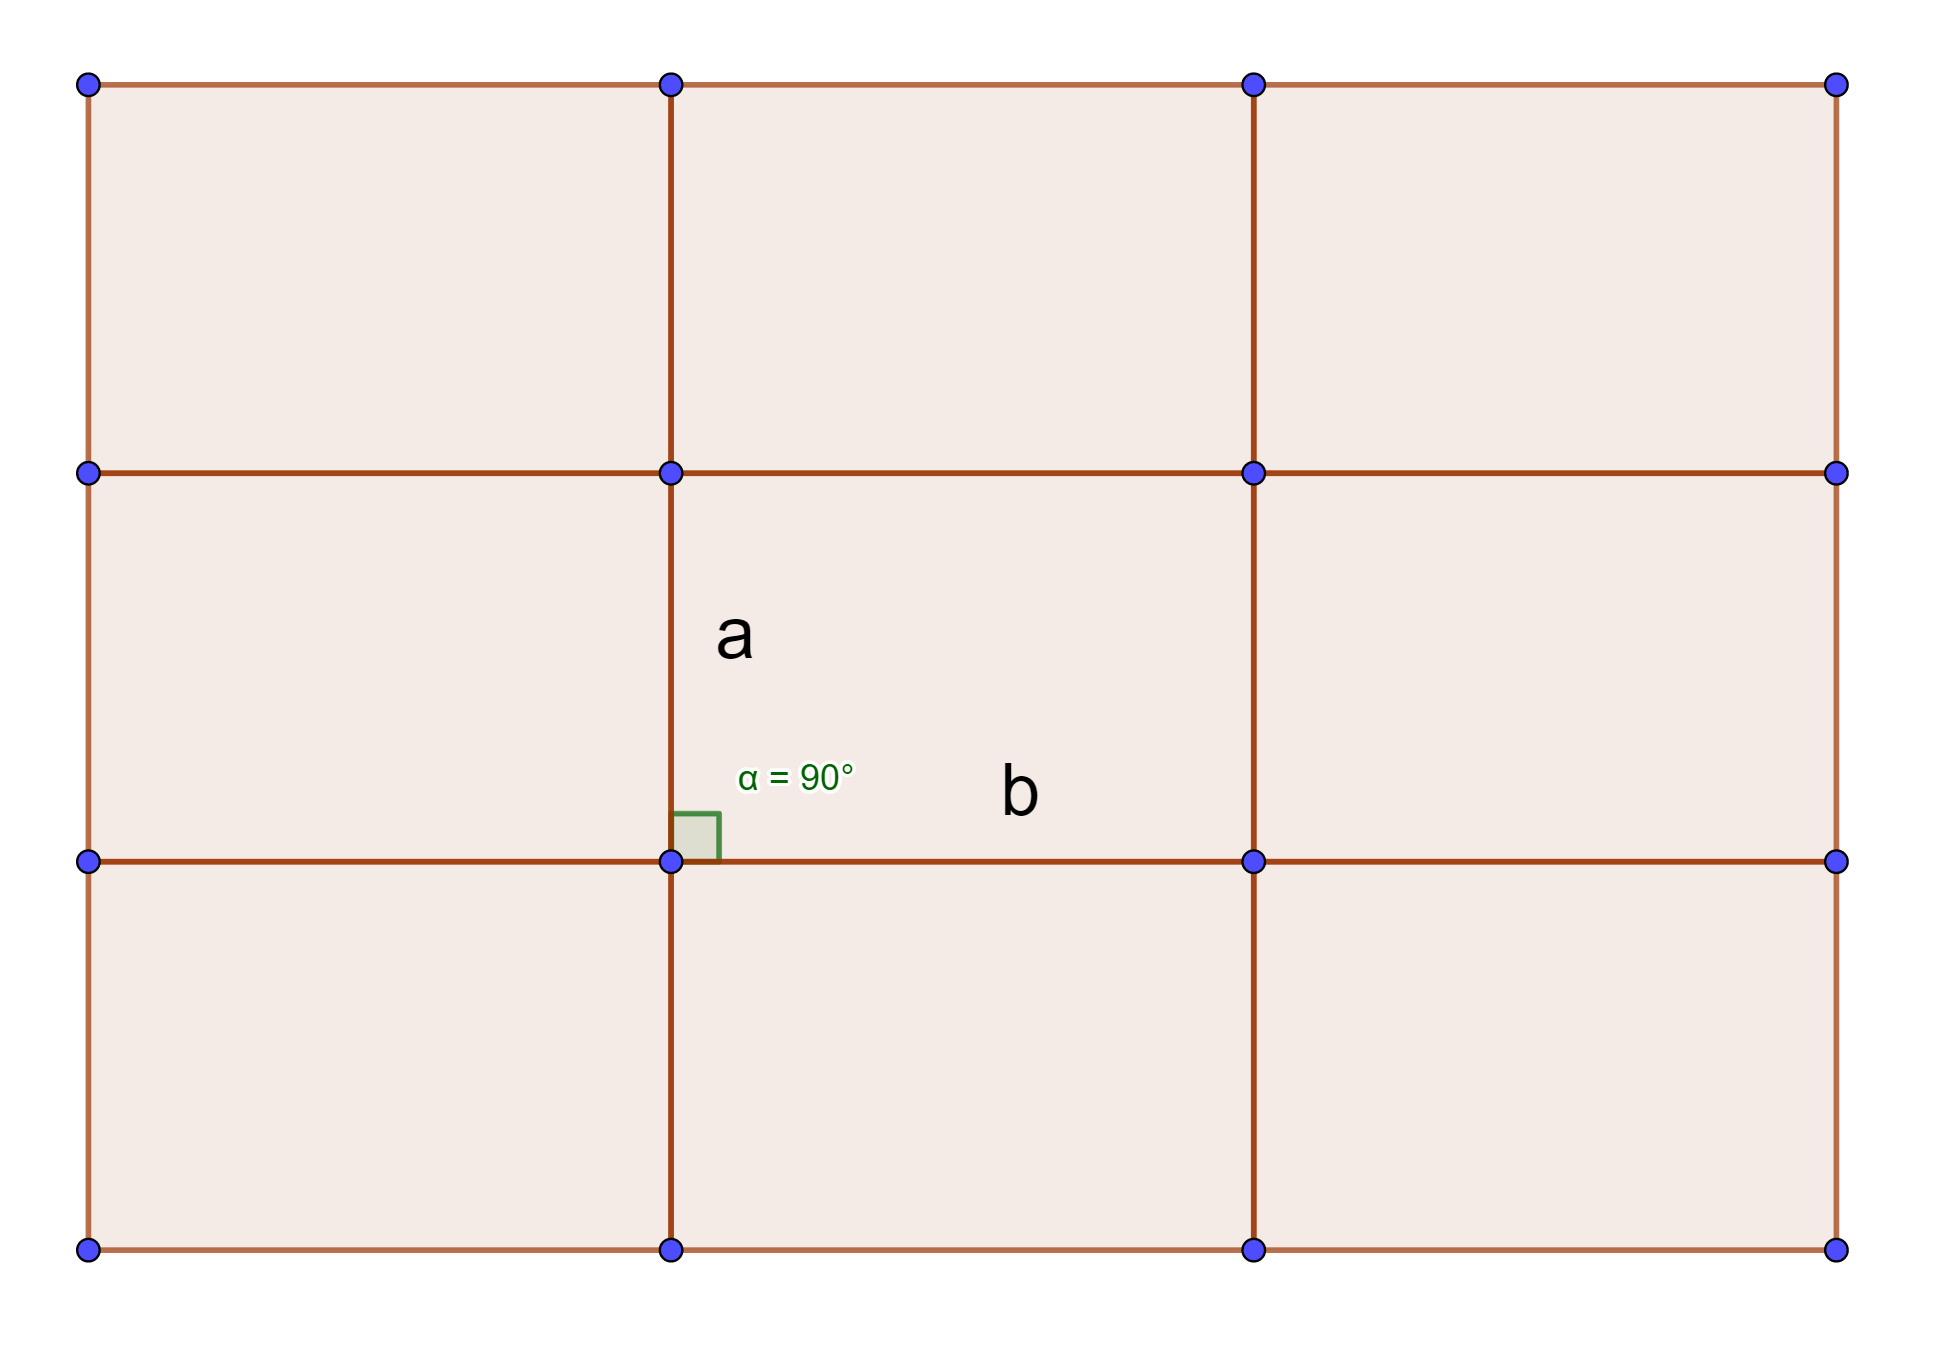
\includegraphics[width=0.4\textwidth]{./pic/p008-2.png}
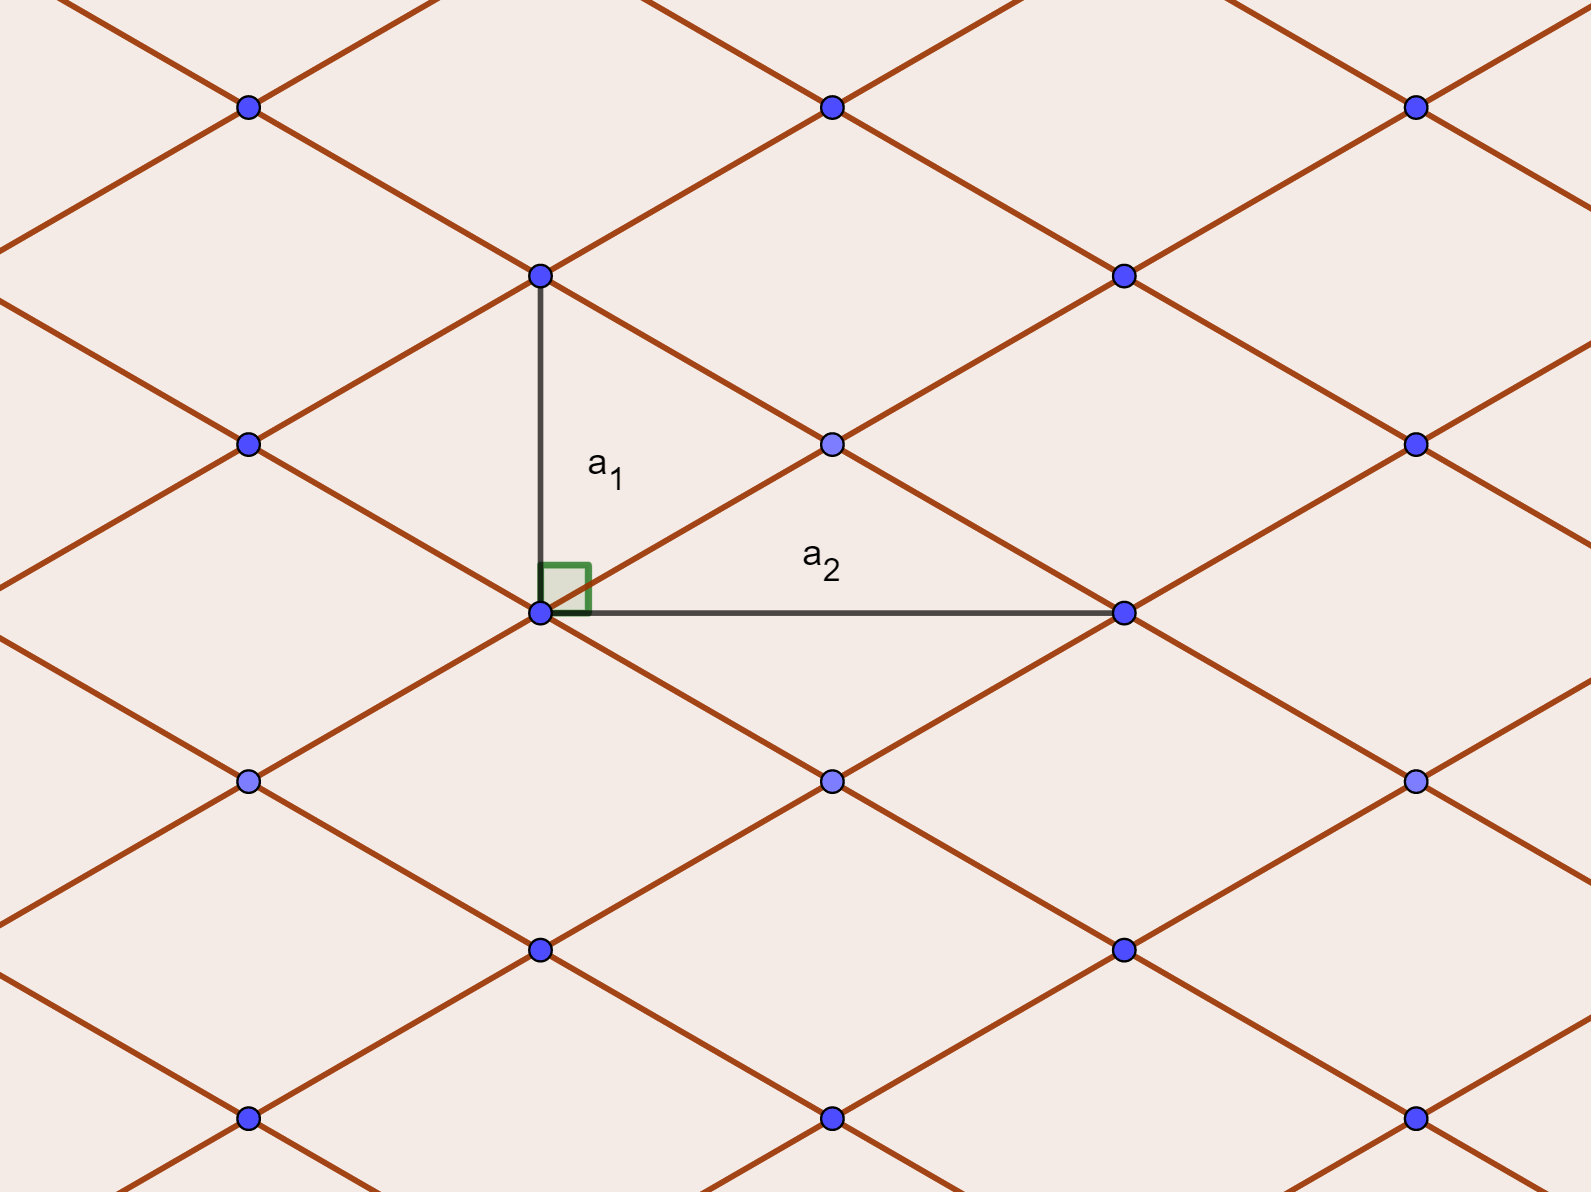
\includegraphics[width=0.3\textwidth]{./pic/p008-3.png}
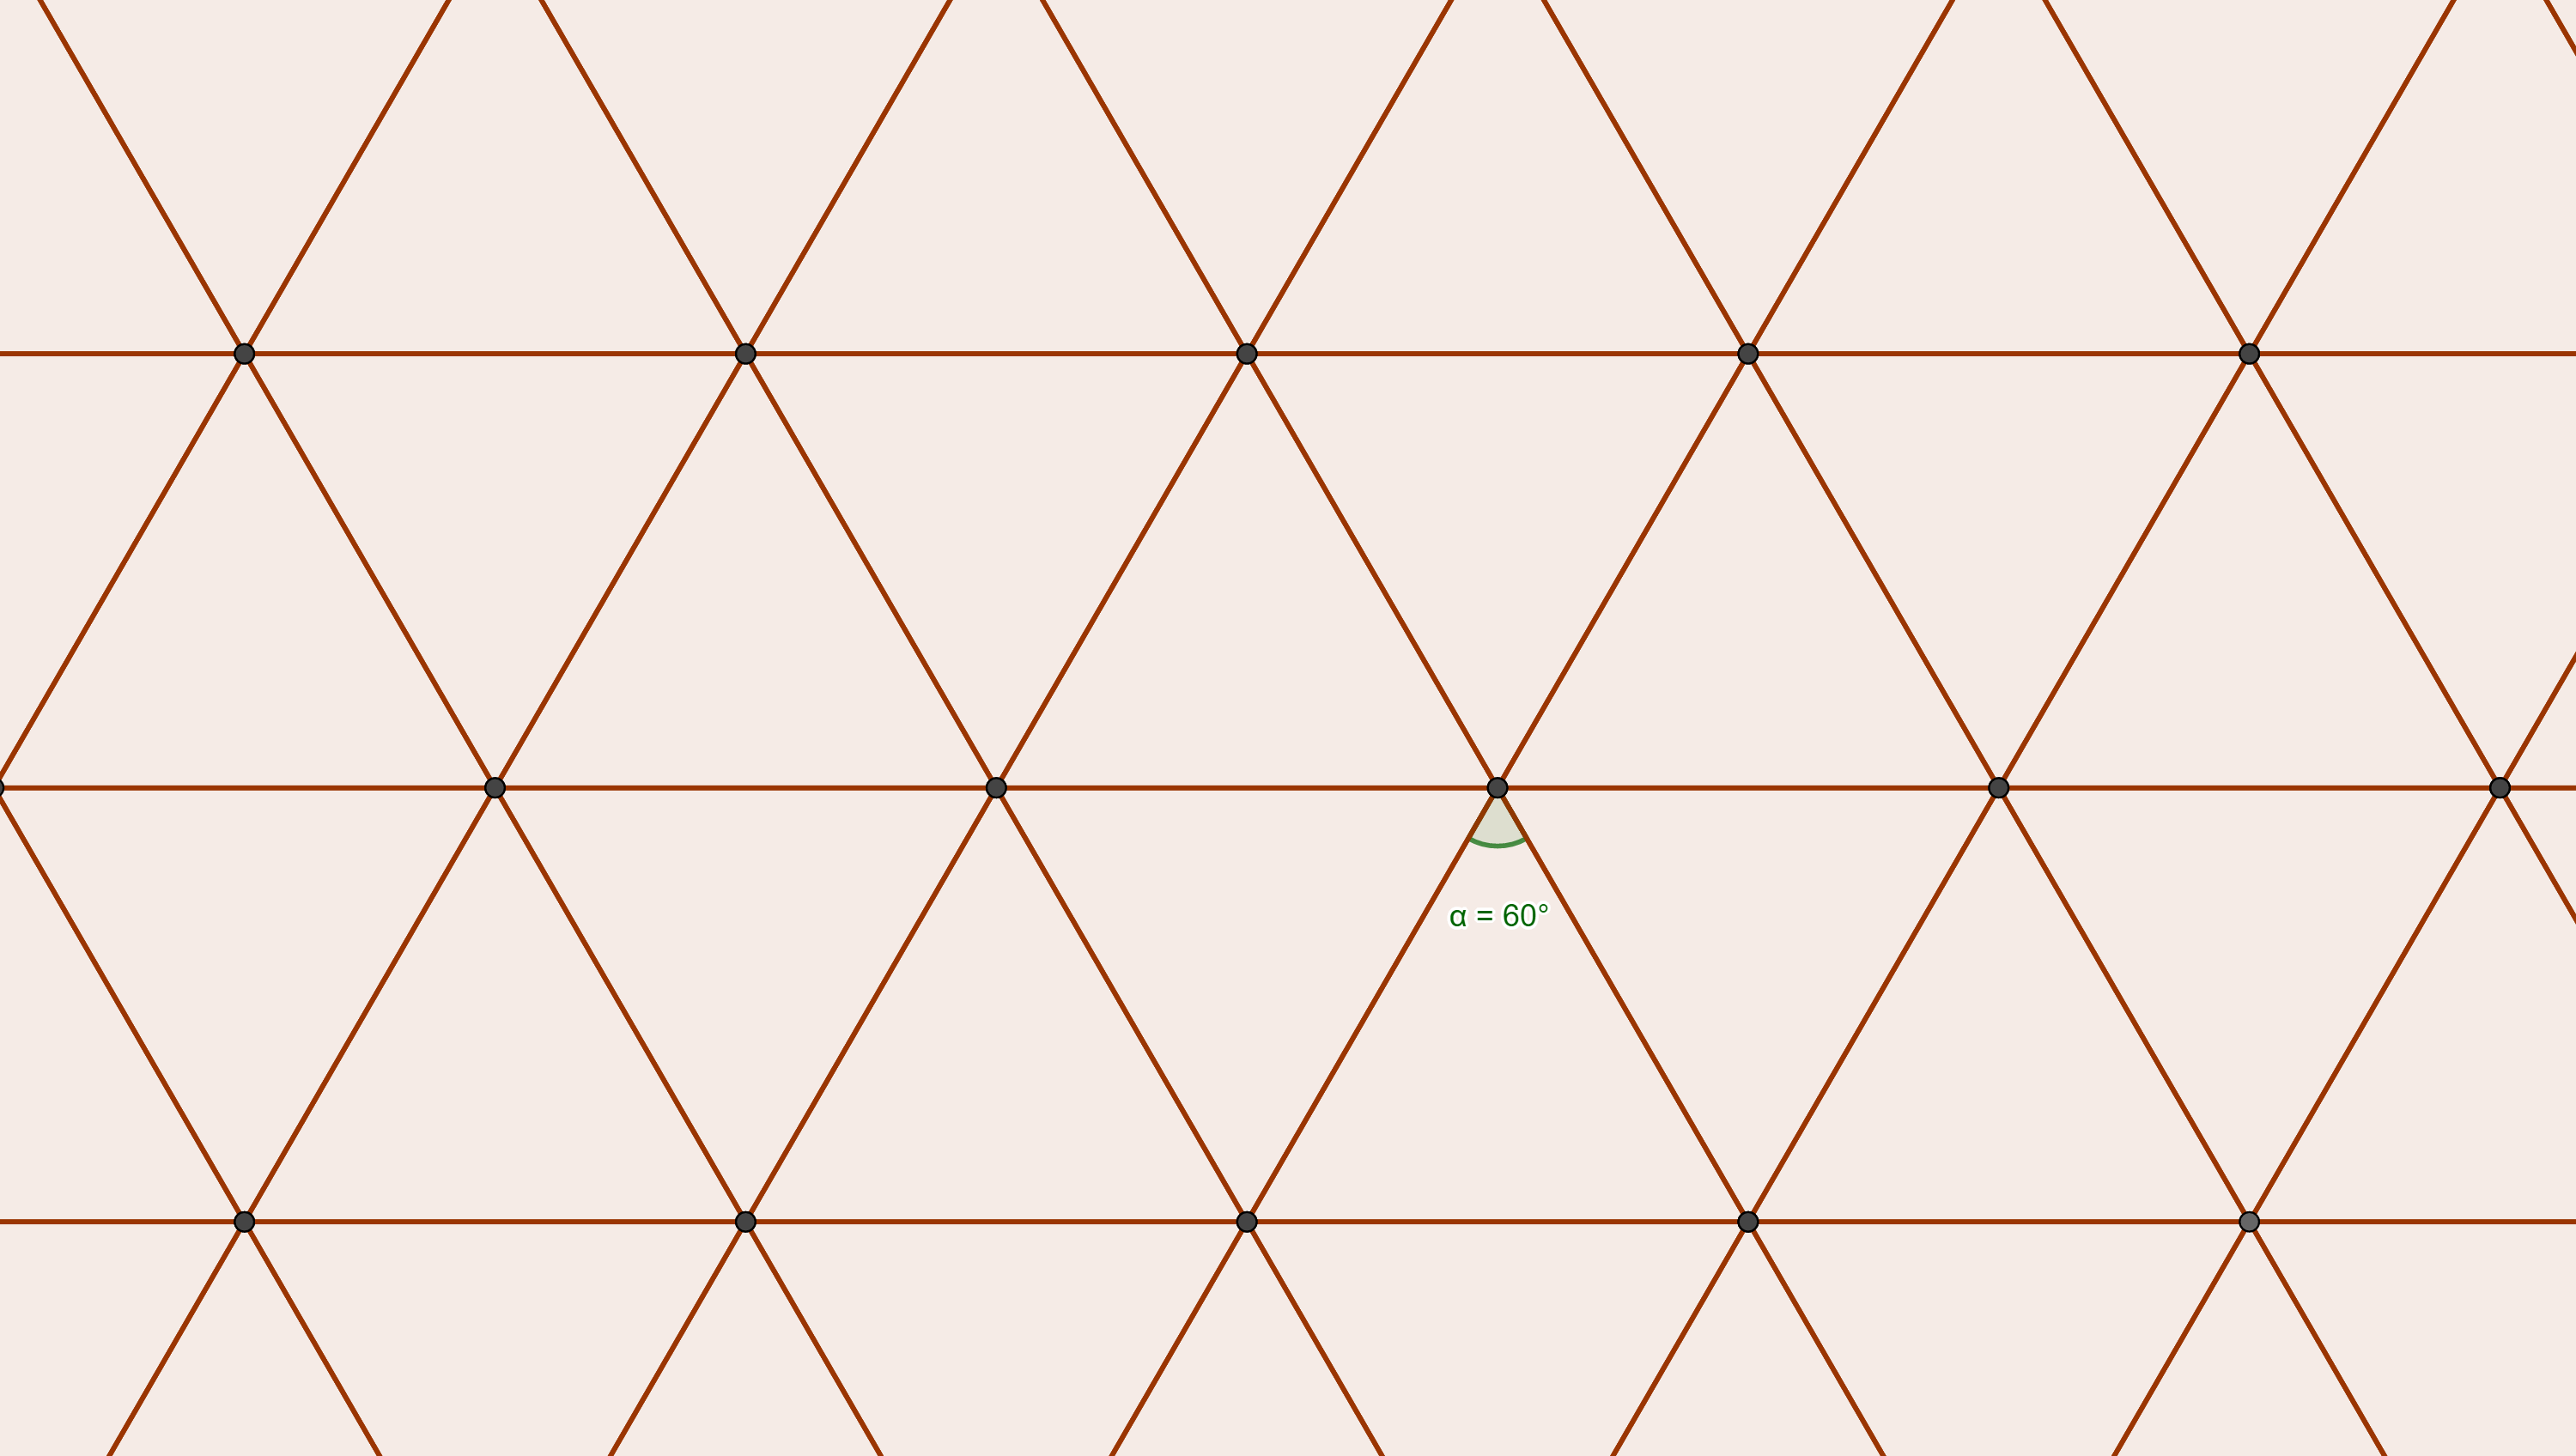
\includegraphics[width=0.3\textwidth]{./pic/p008-4.png}
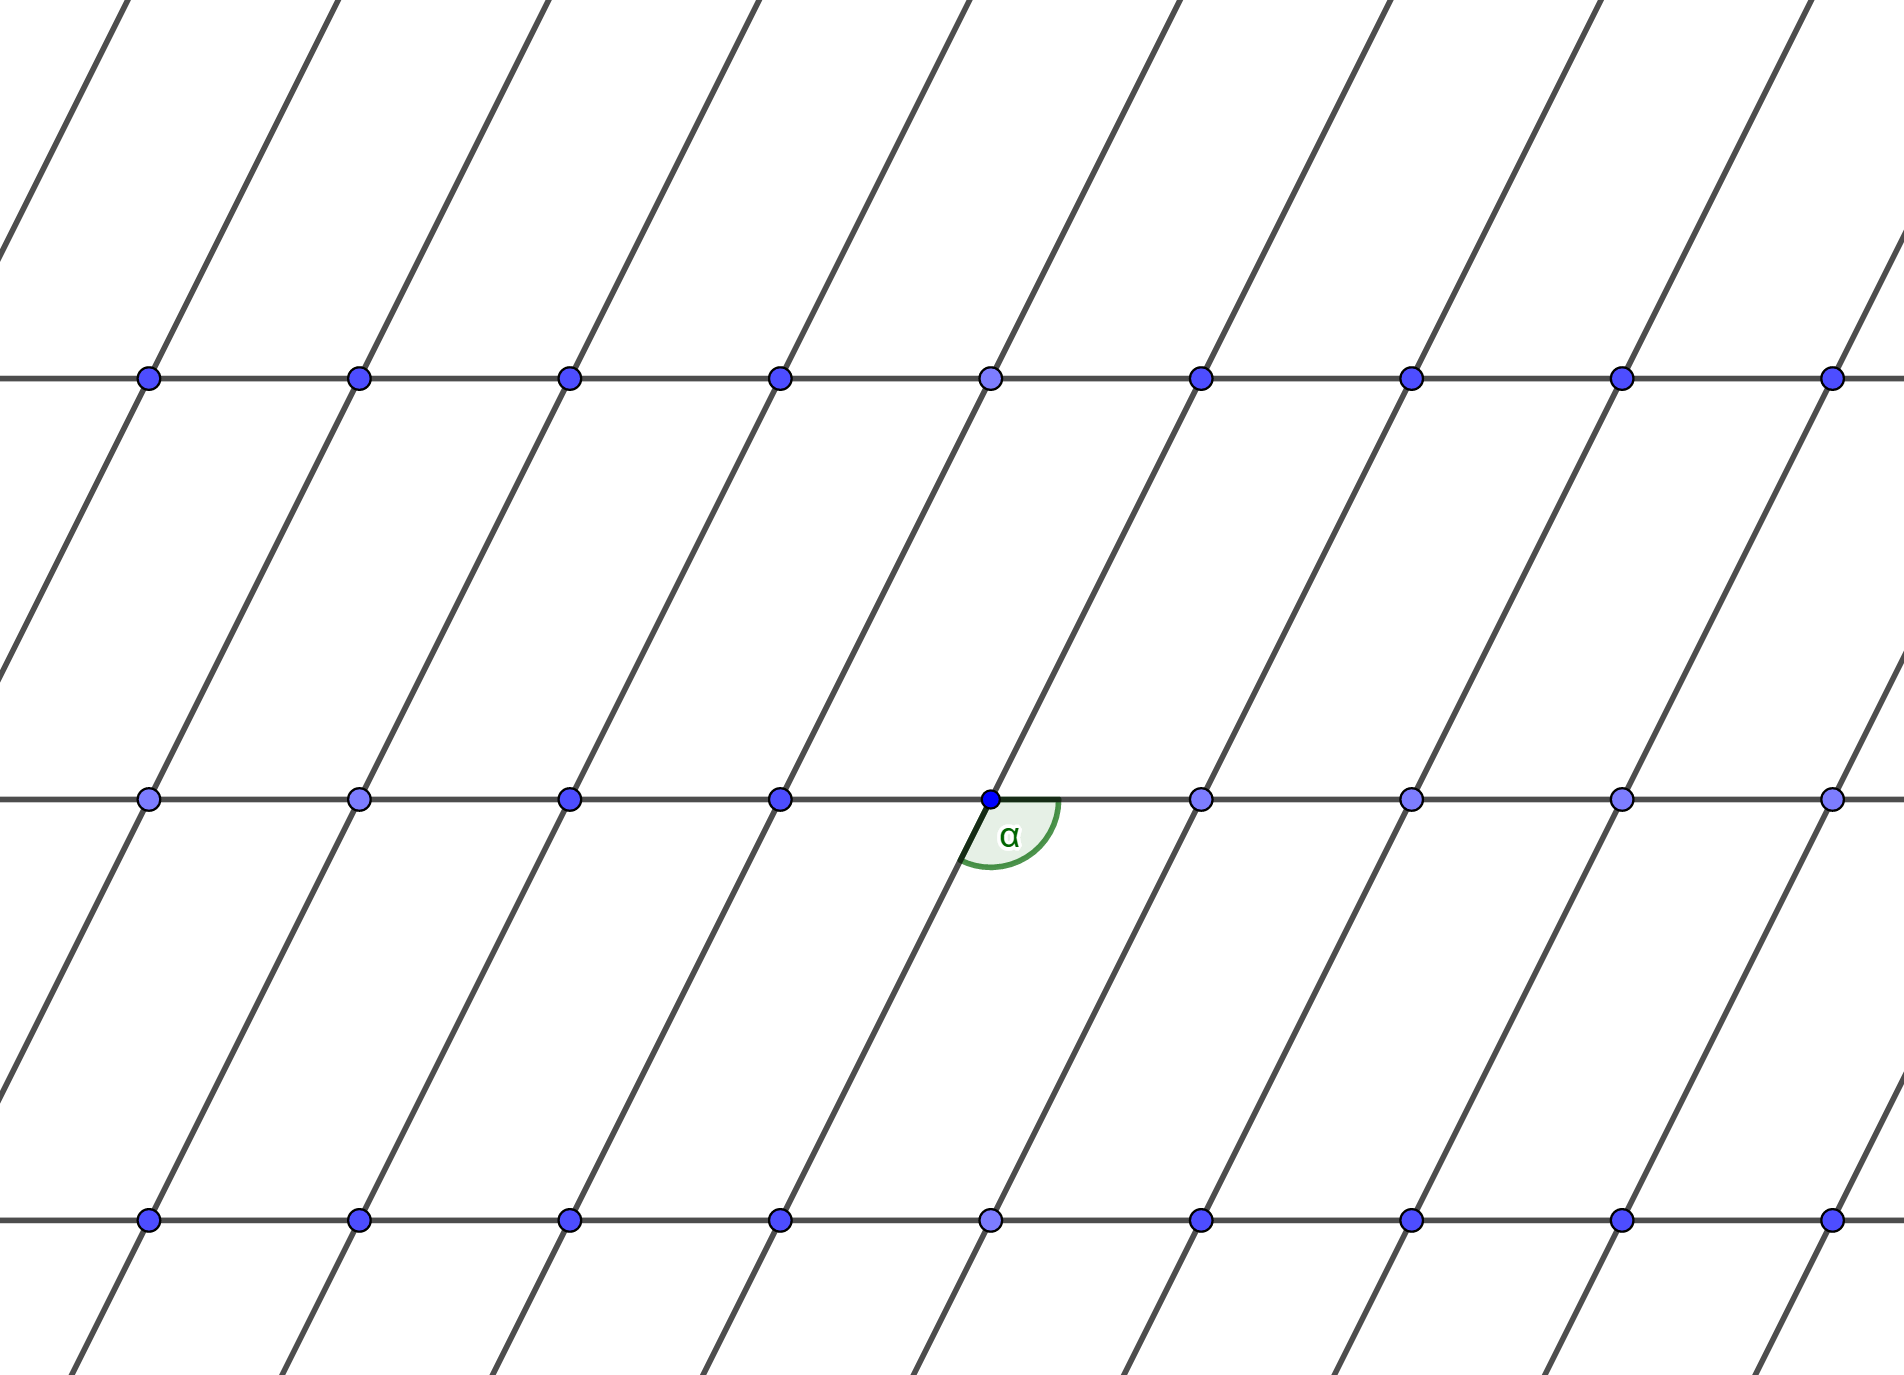
\includegraphics[width=0.3\textwidth]{./pic/p008-5.png}

\caption{JT效应使得氧八面体发生畸变}

\label{dogp02}
\end{figure}
\end{document}